\begin{comment}
\documentclass[10pt]{article}
\usepackage{fullpage, graphicx, url}
\setlength{\parskip}{1ex}
\setlength{\parindent}{0ex}
\title{GEN02}
\begin{document}


\begin{tabular}{ccc}
The Alternative Csound Reference Manual & & \\
Previous & &Next

\end{tabular}

%\hline 
\end{comment}
\section{GEN02}
GEN02�--� Transfers data from immediate pfields into a function table. \subsection*{Description}


  This subroutine transfers data from immediate pfields into a function table. 
\subsection*{Syntax}


 \textbf{f}
 \# time size 2 v1 v2 v3 ...
\subsection*{Initialization}


 \emph{size}
 -- number of points in the table. Must be a power of 2 or a power-of-2 plus 1 (see \emph{f statement}
). The maximum tablesize is 16777216 (224) points. 


 \emph{v1, v2, v3,}
 etc. -- values to be copied directly into the table space. The number of values is limited by the compile-time variable \emph{PMAX}
, which controls the maximum pfields (currently 1000). The values copied may include the table guard point; any table locations not filled will contain zeros. 


 


\begin{tabular}{cc}
\textbf{Note}
 \\
� &

  If p4 is positive, the table will be post-normalized (rescaled to a maximum absolute value of 1 after generation). A negative p4 will cause rescaling to be skipped. 


\end{tabular}

\subsection*{Examples}


  Here is a simple example of the GEN02 routine. It uses the files \emph{gen02.orc}
 and \emph{gen02.sco}
. It places 12 values plus an explicit wrap-around guard value into a table of size next-highest power of 2. Rescaling is inhibited. Here is its diagram: 


 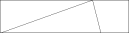
\includegraphics[scale=1]{gen02} 


 Diagram of the waveform generated by GEN02.


 \textbf{Example 1. A simple example of the GEN02 routine.}

\begin{lstlisting}
/* gen02.orc */
; Initialize the global variables.
sr = 44100
kr = 4410
ksmps = 10
nchnls = 1

; Instrument #1.
instr 1
  ; Create an index over the length of our entire note.
  kcps init 1/p3
  kndx phasor kcps

  ; Read Table #1 with our index.
  ifn = 1
  ixmode = 1
  kamp tablei kndx, ifn, ixmode

  ; Create a sine wave, use the Table #1 values to control
  ; the amplitude. This creates a sound with a long attack.
  a1 oscil kamp*30000, 440, 2
  out a1
endin
/* gen02.orc */
        
\end{lstlisting}
\begin{lstlisting}
/* gen02.sco */
; Table #1: an envelope with a long attack (using GEN02).
f 1 0 16 2 0 1 2 3 4 5 6 7 8 9 10 11 0
; Table #2, a sine wave.
f 2 0 16384 10 1

; Play Instrument #1 for 2 seconds.
i 1 0 2
e
/* gen02.sco */
        
\end{lstlisting}
\subsection*{See Also}


 \emph{GEN17}

\subsection*{Credits}


 December 2002. Thanks to Rasmus Ekman, corrected the limit of the \emph{PMAX}
 variable.
%\hline 


\begin{comment}
\begin{tabular}{lcr}
Previous &Home &Next \\
GEN01 &Up &GEN03

\end{tabular}


\end{document}
\end{comment}
